% !TeX spellcheck = en_GB
\documentclass[9pt,twocolumn,twoside,lineno]{pnas-new}
% Use the lineno option to display guide line numbers if required.

\templatetype{pnasresearcharticle}

\title{Public Perceptions on the Coal Debate on Twitter: Reactions to a Corporate Decision-Making Policy Process}

% Use letters for affiliations, numbers to show equal authorship (if applicable) and to indicate the corresponding author
\author[a,b,1]{Yuan Ting Lee}

\affil[a]{Hertie School, Friedrichstr. 180, Berlin 10117, Germany}
\affil[b]{Mercator Research Institute on Global Commons and Climate Change, Torgauer Str. 12 - 15, Berlin 10829, Germany}

% Please give the surname of the lead author for the running footer
\leadauthor{Lee} 

% Please include corresponding author, author contribution and author declaration information
\authorcontributions{}
\authordeclaration{}
\equalauthors{}
\correspondingauthor{\textsuperscript{1}To whom correspondence should be addressed. E-mail: y.lee@mpp.hertie-school.org}

% Keywords are not mandatory, but authors are strongly encouraged to provide them. If provided, please include two to five keywords, separated by the pipe symbol, e.g:
\keywords{Keyword 1 $|$ Keyword 2 $|$ Keyword 3 $|$ ...} 

\begin{abstract}
Please provide an abstract of no more than 250 words in a single paragraph. Abstracts should explain to the general reader the major contributions of the article. References in the abstract must be cited in full within the abstract itself and cited in the text.
\end{abstract}

\dates{This manuscript was compiled on \today}

\begin{document}

\maketitle
\thispagestyle{firststyle}
\ifthenelse{\boolean{shortarticle}}{\ifthenelse{\boolean{singlecolumn}}{\abscontentformatted}{\abscontent}}{}

\dropcap{M}ulti-stakeholder commissions have been an important instrument for incorporating external expertise into political decision-making in Germany. It can be seen as an element of ``negotiation democracy”, whereby the experts in the commission decide on an outcome via deliberations and negotiations. Depending on the policy field, representatives of business, science, the social partners, churches, associations and societies can be appointed and thus accelerate the later public discussion. \cite{Siefken2016}

The Coal Commission, formally known as the Commission on Growth, Structural Change and Employment, is such an example of expert commissions. It was set up by the German government under the Federal Ministry for Economy and Energy (BMWi), and was tasked with developing an overarching approach to managing the coal phase-out’s technical, legal, economic and social impacts.

Criticisms have emerged about the process of the coal commission, namely that ....

The process of the German coal commission thus presents a unique situation for analysis: is there a relationship between the seemingly ``corporatist” process of such an expert commission and public opinion, as represented on social media, on the topic? Here, tweets from Twitter are used to represent public opinion on social media, in part due to their high granularity which allows for observations on swiftly changing temporal patterns on topic salience.

Bacon ipsum dolor amet hamburger tenderloin shoulder chislic, meatball filet mignon venison picanha fatback burgdoggen pork loin kielbasa. Short ribs capicola turducken tenderloin bresaola beef sirloin chicken cow bacon. Pork chop strip steak pastrami ham hock burgdoggen pork loin bresaola leberkas short ribs. Tenderloin ham capicola boudin chicken bacon brisket biltong porchetta chislic kielbasa. Landjaeger andouille tenderloin leberkas hamburger buffalo strip steak bresaola turducken. Beef ribs ground round hamburger prosciutto venison kielbasa swine andouille boudin ham jerky rump filet mignon ham hock. Venison chicken burgdoggen cow, rump shank pork loin frankfurter flank short loin.

Porchetta chislic tongue chicken brisket strip steak burgdoggen swine leberkas fatback drumstick picanha frankfurter capicola. Pork loin t-bone ground round, pig short ribs drumstick beef tenderloin swine. Tenderloin corned beef jerky burgdoggen sausage pork chop boudin landjaeger rump swine chicken. Alcatra short loin pork, hamburger tongue jerky shoulder buffalo rump filet mignon ball tip.

\section*{Related Work}
Meatloaf short ribs pork chop boudin. Kielbasa turkey landjaeger, strip steak leberkas alcatra chislic cupim prosciutto porchetta tri-tip brisket swine short loin. Drumstick bacon capicola picanha tail filet mignon. Brisket andouille spare ribs, beef ribeye hamburger pastrami shankle frankfurter fatback filet mignon. Buffalo filet mignon salami chicken sirloin ham jowl short ribs.

Hamburger turducken biltong, leberkas brisket alcatra ribeye buffalo ham salami jowl. Short ribs ribeye chicken, chislic prosciutto brisket kielbasa pancetta porchetta buffalo. Tenderloin turducken boudin short loin tongue porchetta. Tail flank shankle porchetta alcatra picanha shank jerky ham biltong. Ball tip flank filet mignon sausage. Jowl spare ribs buffalo corned beef ham hock, landjaeger ground round porchetta ham.

Ribeye ground round pork, biltong shankle turducken chuck alcatra pancetta rump landjaeger. Rump bacon tongue buffalo. Cow landjaeger alcatra ground round pancetta shankle filet mignon picanha leberkas pork chicken. Pastrami pork pork chop, chicken kevin pig shoulder. Ground round flank jowl kielbasa shank cow. Corned beef pork loin meatball, short loin ground round bresaola pig rump jowl hamburger meatloaf boudin brisket shankle andouille.

Twitter has been used as a medium to analyse human sentiment through the analysis of variations in the frequency of specific words used by individuals. In \cite{Dodds2011}, Dodds et. al. develop a tool for measuring expressed happiness via positive and negative sentiment in large-scale text corpora. Since its development, the tool, named the ``hedonometer”, has been implemented in studies involving the happiness of cities and states, the happiness of the English language as a whole, the relationship between individuals' happiness and that of those they connect with, and as a method of unsolicited public opinion polling on climate change. % cite cite !

\section*{Task}


\section*{Data}
The data used in this project was collected via a two-part process, using two python packages: \texttt{twint} to download the tweets based on specific queries, and \texttt{tweepy} to populate the tweets with extended tweet information. %be more specific and clear here

% insert figure on data collection

The selection process for choosing tweets to analyse stems from the research question at hand, which is to understand the greater coal debate in Germany on Twitter. The final collection of tweets thus include two sets of tweets collected using two different search strategies. The first search strategy includes terms that directly relate to the coal exit in Germany - \{Kohlekommission, Kohleausstieg, Kohlefrei\}.\footnote{Translation: Coal commission, Coal exit, Coal free}

The other set of tweets is obtained from a general search for tweets on coal ("Kohle"), which are then filtered by the inclusion of relevant hashtags in the text of the tweets. These relevant hashtags are obtained by conducting a frequency analysis of all hashtags that appear in "Kohle" tweets, and manually selecting the top hashtags that are related to coal in climate policy. These hashtags are:  \{\#Klimaschutz, \#Hambacherforst, \#Hambibleibt, \#endcoal, \#fridaysforfuture, \#klimawandel, \#klima, and \#endegelaende\}.\footnote{Translation: Climate policy, Hambach Forest, Stay Hambach (forest), Climate Change, Climate, End of the Site} 

The two collections are then combined and duplicates are removed, and the final set is then filtered for tweets in German, which can be obtained as a result from querying the Twitter API. 

\begin{figure} 
	\begin{center}
		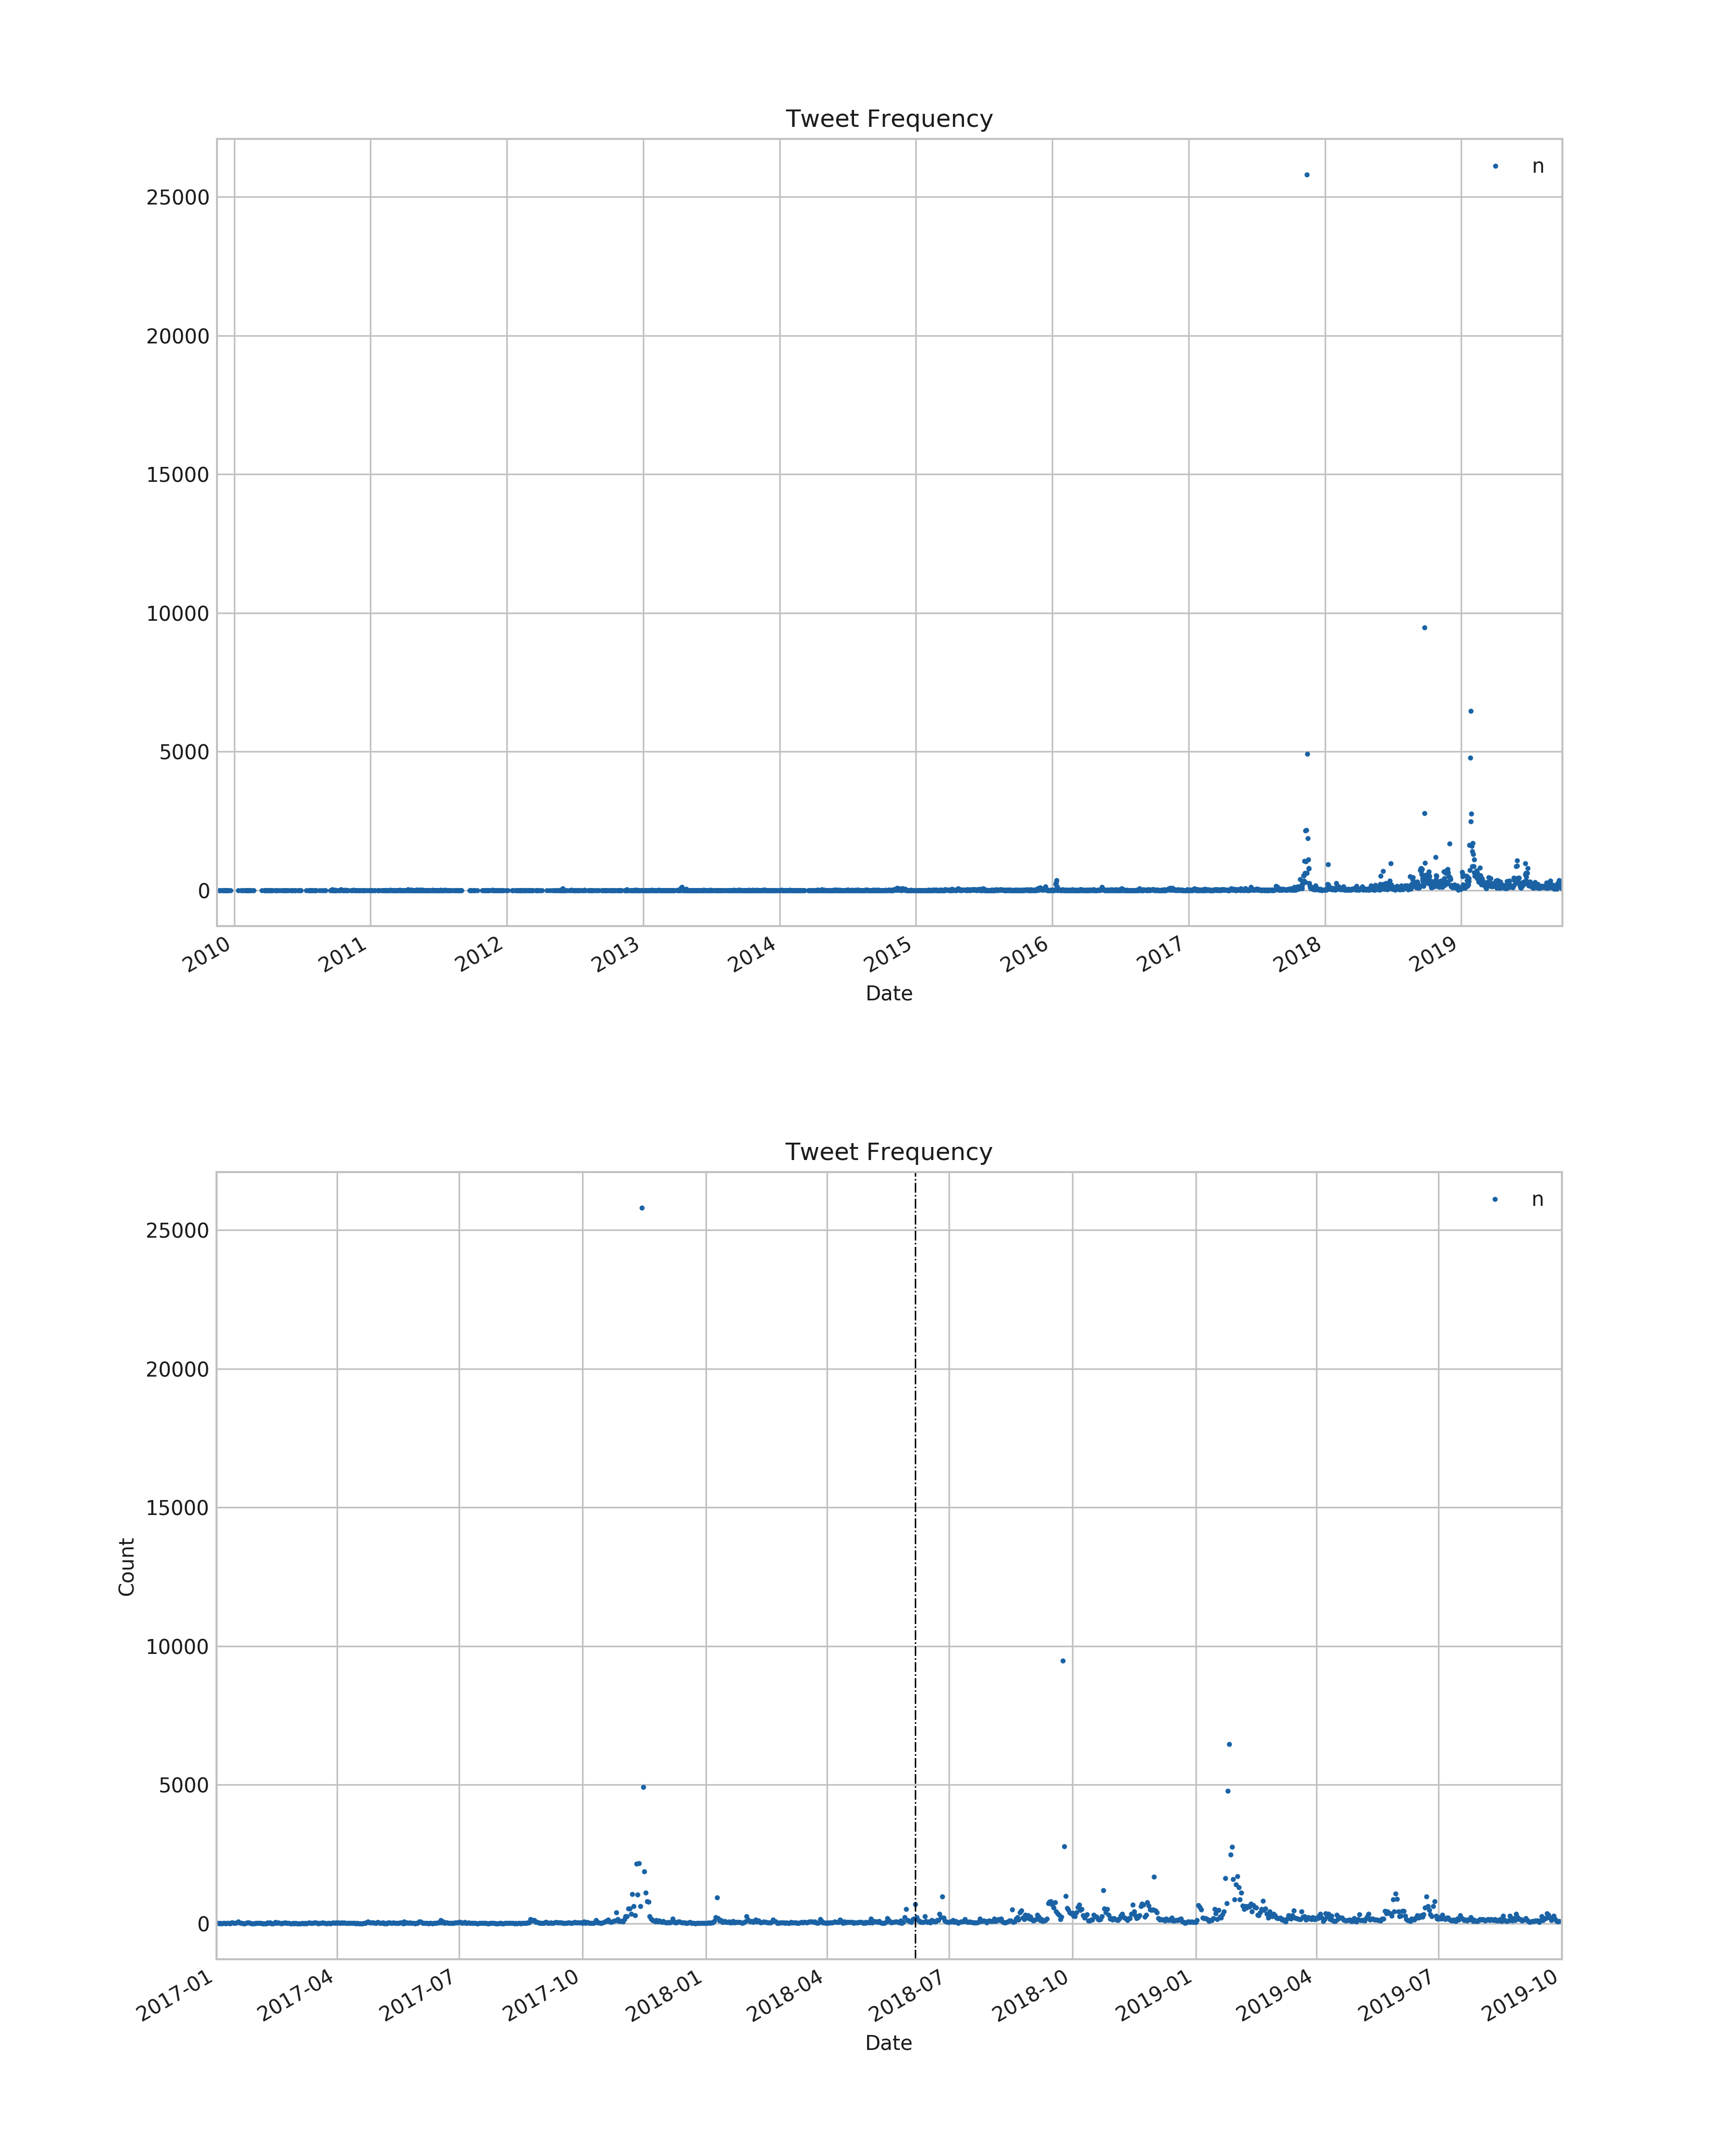
\includegraphics[width=\linewidth]{figures/tweet_frequency_combine}
	\end{center}
	\caption{Daily frequency of tweets in combined dataset, over entire collection period and over coal commission process}
	\label{fig:tweet_frequency}
\end{figure}

\section*{Proposed Method}
\subsection*{Sentiment Analysis}
% Explanation of sentiment analysis 

Sentiment analysis refers to the use of natural language processing and text analysis to systematically identify and extract affective states and subjective information in text. % cite?

The dictionary used is SentiWS, a publicly available German-language resource for sentiment analysis. \cite{REMUS10.490} Entries in the SentiWS dictionary set have four components: the word, its Part of Speech (POS) tag, a polarity weight, and inflections associated with the word, as seen in Fig. \ref{fig:sentiws_example}. The semantic orientations of the words are obtained from three different sources with manual revision. 

The weights of word entries in SentiWS are retrieved using a method known as \emph{Pointwise Mutual Information} (PMI), first suggested in \cite{church-hanks-1990-word}. This approach was successfully re-used for sentiment analysis -- the determination of the semantic orientation and the strength of adjectives -- in \cite{Turney2002} and \cite{Turney2003}, where semantic orientation is inferred from \emph{semantic association}. The semantic orientation \(SO\) of a given word \(w\) is calculated from the strength of its association \(A\) with a manually-selected set of positive seed words \(P\) minus the strength of its association with a set of negative seed words \(N\) (cf. Equation \ref{eq:semantic_orientation}). 

\begin{equation}
\label{eq:semantic_orientation}
\text{SO-A}(w) = \sum_{p \in P}A(w,p) - \sum_{n \in N}A(w,n)
\end{equation}

The word \(w\) is classified as having a positive semantic orientation when SO-A\(w\) is positive and a negative semantic orientation SO-A\(w\) is negative. The absolute value of SO-A\(w\) can be considered the strength of its semantic orientation. 

Parallel to the paradigms in \cite{Turney2003}, SentiWS uses a set of German seed words, from which the semantic associations \(A(w,p)\) and \(A(w,n)\) are calculated using PMI (Equation \ref{eq:pmi}): 

\begin{equation}
\label{eq:pmi}
\text{PMI}(w_1,w_2) = \log_2\left(\frac{P(w_1 \& w_2)}{P(w_1) \cdot P(w_2)}\right)
\end{equation}
where \(P(w)\) is the probability that \(w\) occurs and \(P(w_1 \& w_2)\) is the probability that \(w_1\) and \(w_2\) co-occur. The probabilities were estimated using frequencies and co-occurrence statistics on an internal German-language corpus by the creators of SentiWS consisting of approximately 100 Million sentences.  

\begin{figure} 
	\begin{center}
		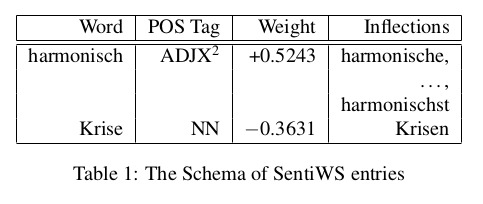
\includegraphics[width=\linewidth]{figures/sentiws_example}
	\end{center}
	\caption{Schema of SentiWS entries}
	\label{fig:sentiws_example}
\end{figure}

To obtain the sentiment score of a tweet, denoted by \(s_{tweet}\), the following formula is used: 

\begin{equation}
\label{eq:word_score}
s_{tweet} = \frac{\sum_{i=1}^{n} s_i f_i}{\sum_{i=1}^{n} f_i}
\end{equation} 
where \(s_i\) is the polarity weighting score of a word given in SentiWS, and \(f_i\) is the frequency of occurrence of the word in the tweet. 



\section*{Results}

\begin{figure} 
	\begin{center}
		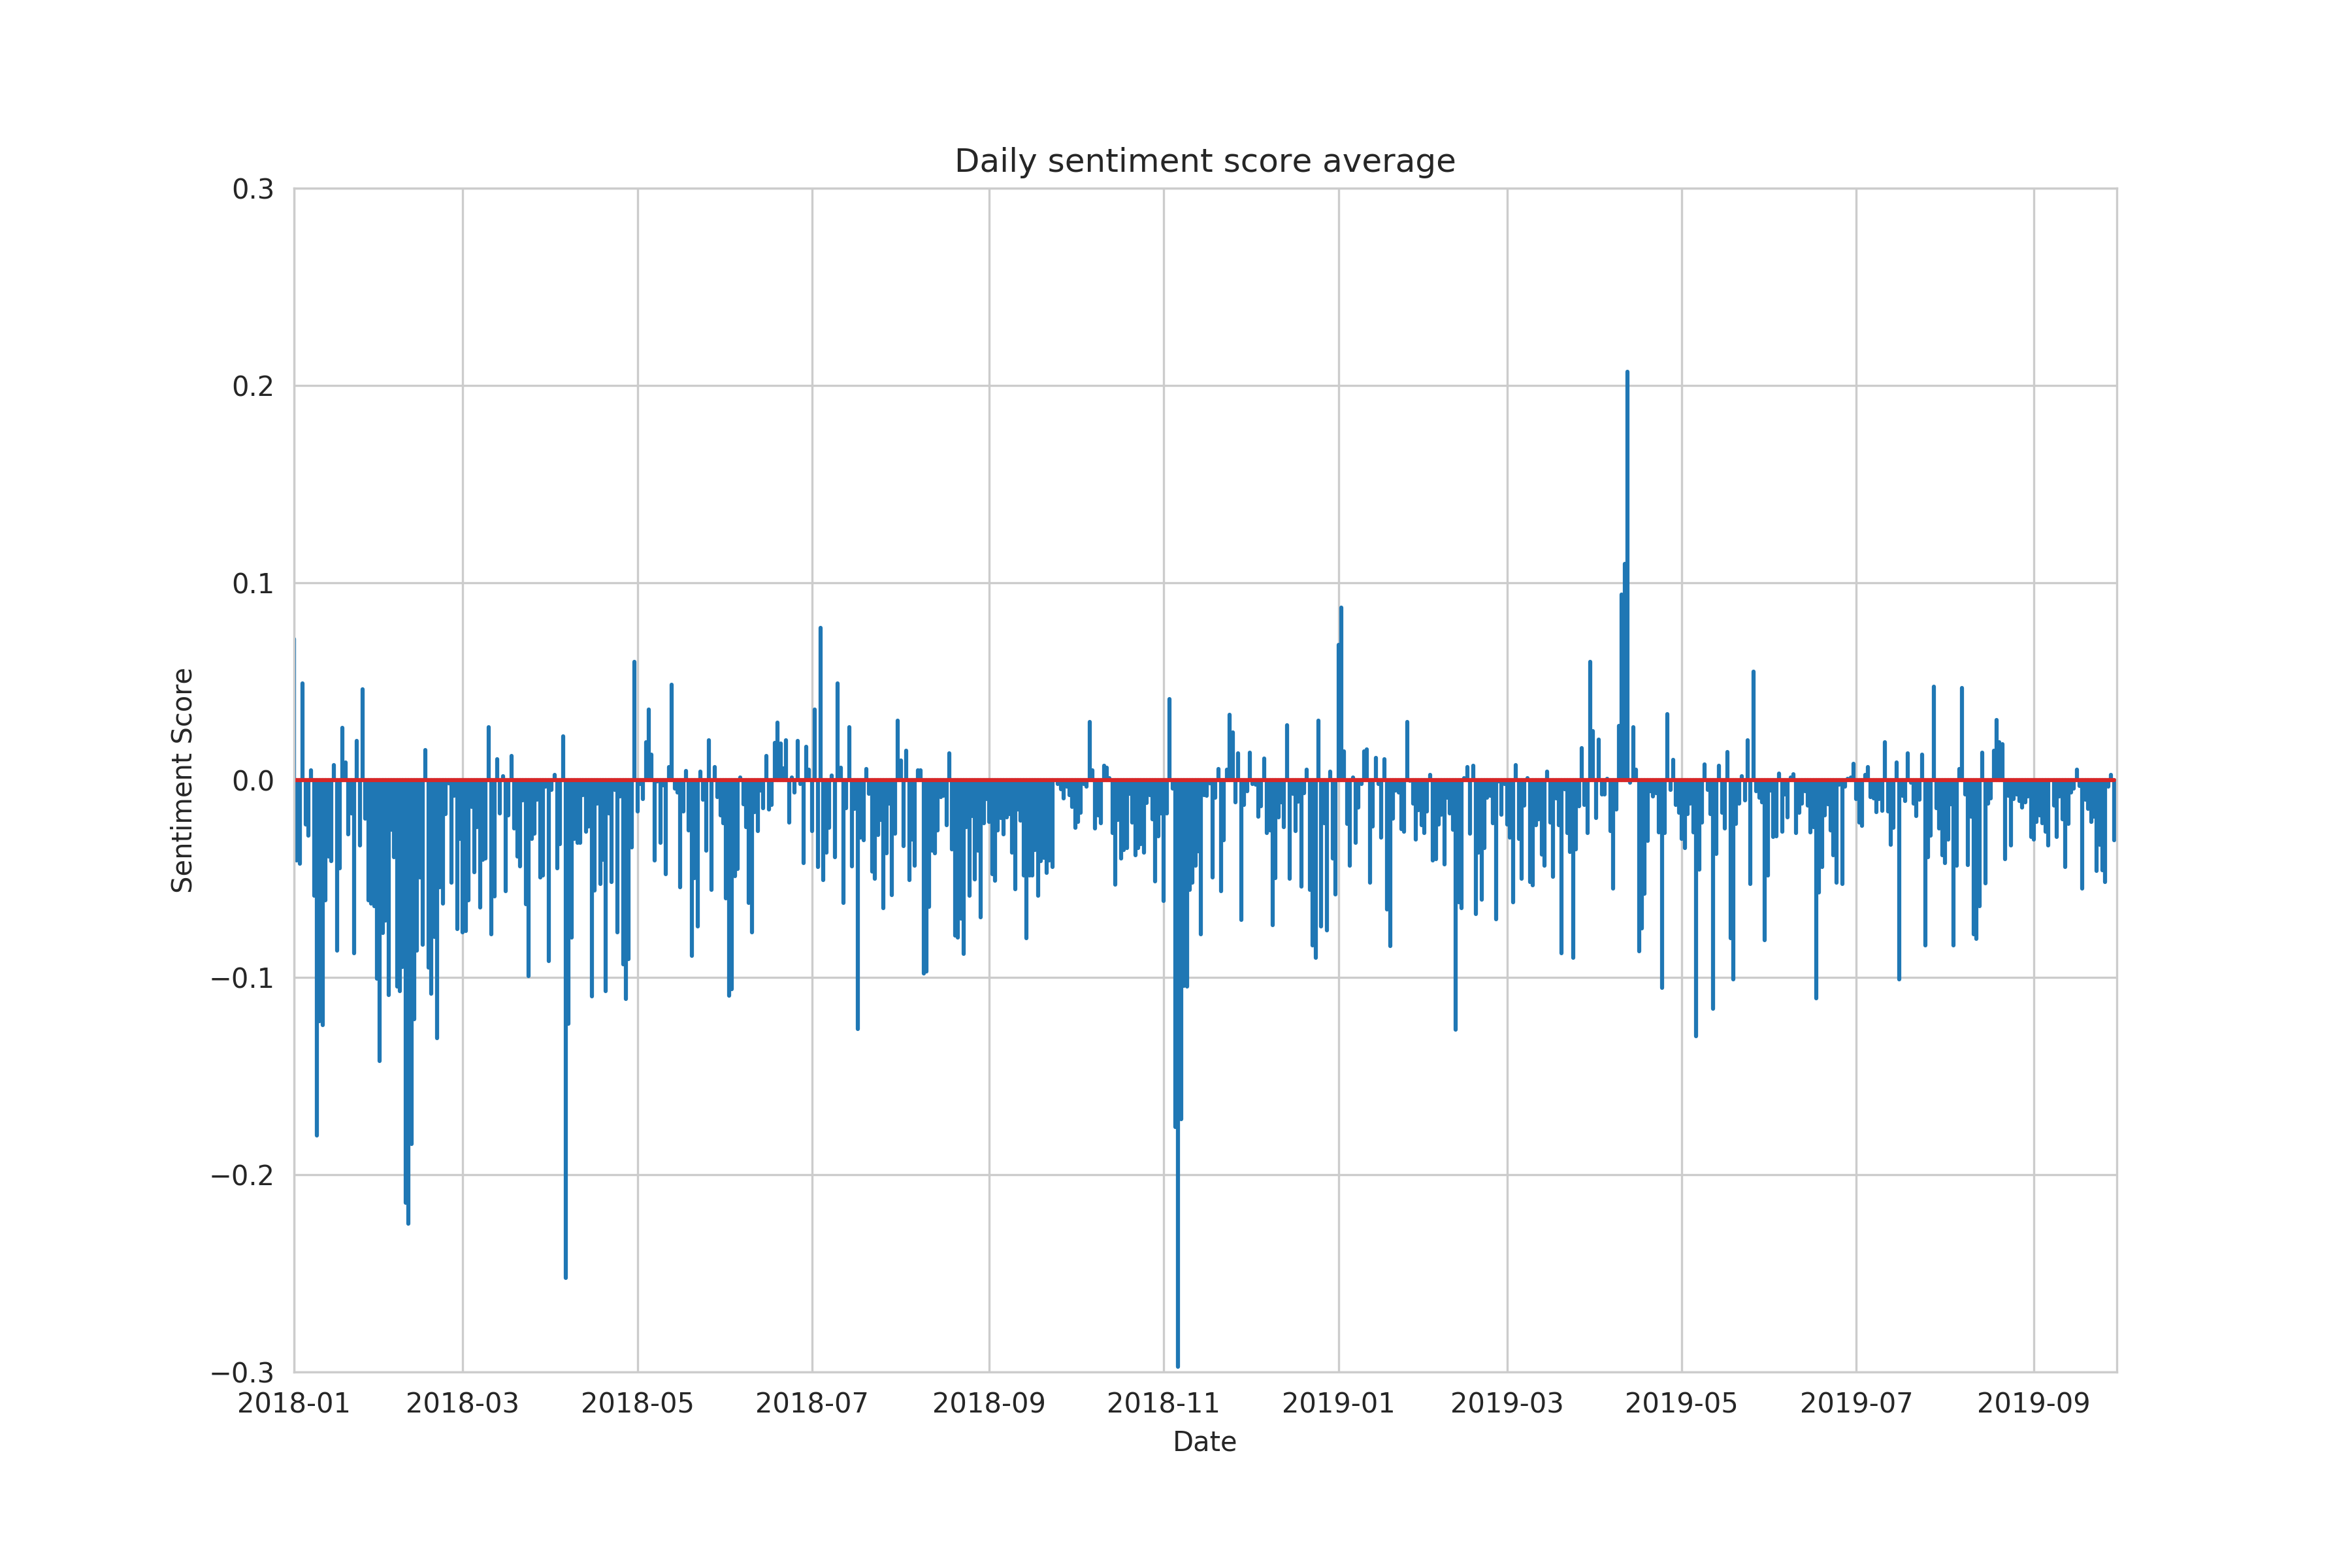
\includegraphics[width=\linewidth]{figures/dailyavgsenti}
	\end{center}
	\caption{Daily average sentiment score of tweets}
	\label{fig:tweet_score}
\end{figure}



\subsubsection*{Event Analysis} 


\subsubsection*{Word Shift}


\subsubsection*{Network Analysis}



\section*{Discussion}


\acknow{Please include your acknowledgments here, set in a single paragraph. Please do not include any acknowledgments in the Supporting Information, or anywhere else in the manuscript.}

\showacknow{} % Display the acknowledgments section

\section*{References}
% Bibliography
\bibliography{bibliography.bib}

\end{document}